\setcounter{ex}{0}
\section{Đường tiệm cận của đồ thị hàm số}
\subsection{Đề 1}
\Opensolutionfile{ans}[ans/ans-2-B3-De1-lc]
\caulc
\begin{ex}%Câu 1%[2D1N4-1]
	\immini[thm]
	{Cho hàm số $f(x)$ xác định trên $\mathbb{R}\setminus \{-1\}$, liên tục trên mỗi khoảng xác định và có đồ thị như hình vẽ sau. Mệnh đề nào dưới đây đúng?
	\choice[1]
	{Đồ thị hàm số đã cho không có tiệm cận đứng}
	{\True Đồ thị hàm số đã cho có đúng một tiệm cận đứng là đường thẳng $x=-1$}
	{Đồ thị hàm số đã cho có đúng một tiệm cận đứng là đường thẳng $x=2$}
	{Đồ thị hàm số đã cho có hai tiệm cận đứng là các đường thẳng $x=-1$ và $x=2$}
	}
	{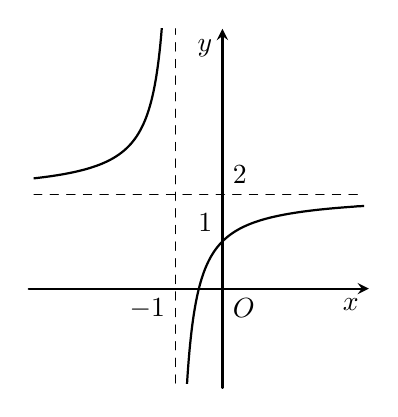
\begin{tikzpicture}[line join=round, line cap=round,>=stealth,thick,scale=0.6]
			\draw[->] (-4.1,0)--(3.1,0) node[below left] {$x$};
			\draw[->] (0,-2.1)--(0,5.5) node[below left] {$y$};
			\draw (0,0) node [below right] {$O$};
			\draw[dashed,thin] (-0.99,-2)--(-0.99,5.5);
			\begin{scope}
				\clip (-4,-2) rectangle (3,5.5);
				\draw[samples=200,domain=-4:-1.01,smooth,variable=\x] plot (\x,{(2*(\x)+1)/(1*(\x)+1)});
				\draw[samples=200,domain=-0.99:4,smooth,variable=\x] plot (\x,{(2*(\x)+1)/(1*(\x)+1)});
				\draw[dashed,thin] (-4,2/1)--(4,2/1);
			\end{scope}
		\draw(-1,0)node[below left]{$-1$} (0,1)node[above left]{$1$} (0,2)node[above right]{$2$};
	\end{tikzpicture}}
	\loigiai{
Nhìn vào đồ thị ta suy ra tiệm cận đứng là đường thẳng $ x=-1$.}
\end{ex}
\begin{ex}%Câu 2%[2D1H4-1]
\immini[thm]
{Cho hàm số $y=f(x)$ xác định trên $\mathbb{R}\backslash\{1\}$, liên tục trên mỗi khoảng xác định và có đồ thị như hình bên.
	Tiệm cận xiên của đồ thị hàm số $y=f(x)$ là đường thẳng có phương trình
	\choice[2]
	{$ y=2x+1$}
	{$ y=1$}
	{\True $ y=x$}
	{$ y=x+1$}
}
{ 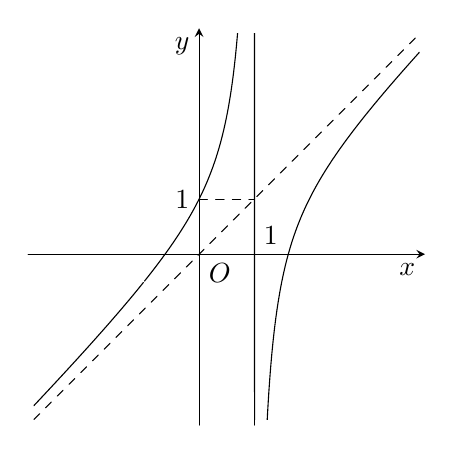
\begin{tikzpicture}[line join=round, line cap=round,>=stealth,scale=0.7]
		\draw[->] (-3.1,0)--(4.1,0) node[below left] {$x$};
		\draw[->] (0,-3.1)--(0,4.1) node[below left] {$y$};
		\draw (0,0) node [below right] {$O$};
		\draw[dashed,thin] (1,-3.1)--(1,4.1);
		\begin{scope}
			\clip (-3,-3) rectangle (4,4);
			\draw[samples=200,domain=-3:-1.01,smooth,variable=\x] plot (\x,{(1*((\x)^2)-1*(\x)-1)/(1*(\x)-1)});
			\draw[samples=200,domain=-0.99:4,smooth,variable=\x] plot (\x,{(1*((\x)^2)-1*(\x)-1)/(1*(\x)-1)});
			\draw[dashed,thin] (-3,-3)--(4,4);
		\end{scope}
	\draw[dashed](0,1)node[left]{$1$}--(1,1);
	\draw(1,0)node[above right]{$1$};
\end{tikzpicture}}
	\loigiai{
Tiệm cận xiên là đường thẳng $d\colon y=ax+b$, $\left(a\ne 0\right)$.\\
Đường thẳng $ d$ đi qua hai điểm $\left(0;0\right)$, $\left(1;1\right)$.\\
Khi đó ta có hệ phương trình $\heva{&0=a\cdot0+b\\&	1=a\cdot1+b}\Rightarrow\heva{&a=1\\&b=1.}$\\
Do đó tiệm cận xiên là đường thẳng $ y=x$.
}
\end{ex}

\begin{ex}%Câu 3%[2D1N4-1]
	Cho hàm số $ y=f(x)$ xác định, liên tục trên $\mathbb{R}$ và thỏa mãn $\displaystyle\lim\limits_{x\to-\infty}y=2$; $ \displaystyle\lim\limits_{x\to2^+}=0$. Khẳng định nào sau đây đúng?
	\choice
	{Đồ thị hàm số có tiệm cận ngang là $ x=2$ và có tiệm cận đứng $ y=2$}
	{\True Đồ thị hàm số có tiệm cận ngang là $ y=2$ và không có tiệm cận đứng}
	{Đồ thị hàm số không có tiệm cận ngang và có tiệm cận đứng $ x=2$}
	{Đồ thị hàm số có tiệm cận ngang là $ y=2$ và có tiệm cận đứng $ x=2$}
	\loigiai{
Theo định nghĩa tiệm cận của đồ thị hàm số.
}
\end{ex}

\begin{ex}%Câu 4%[2D1N4-1]
	\immini[thm]
	{Cho hàm số $y=f(x)$ xác định, liên tục trên $\mathbb{R}$ và có đồ thị như hình bên.
		Tiệm cận ngang của đồ thị hàm số $y=f(x)$ là đường thẳng có phương trình
		\choice[2]
		{$ y=0$}
		{\True $ y=1$}
		{$ y=x$}
		{$ x=1$}}
	{ \begin{tikzpicture}[line join=round, line cap=round,>=stealth,scale=0.7]
			\draw[->] (-5.1,0)--(4.1,0) node[below left] {$x$};
			\draw[->] (0,-2.1)--(0,3.1) node[below left] {$y$};
			\draw (0,0) node [below left] {$O$};
			\draw[thin] (-5,1)--(4,1);
			\begin{scope}
				\clip (-5,-2) rectangle (4,3);
	\draw[name path=f(x)] plot[smooth,tension=0.5] coordinates{(-5,0.85) (-3.5,0.75) (-2.5,0) (-0.9,-1.7) (0,-1) (1.3,2) (2,1.3) (4,1.15) };
			\end{scope}
	 \foreach \x/\nx in {-3/-3,-2/-2,-2/-2,1/1,2/2,3/3}
	 \draw[thin] (\x,1pt)--(\x,-1pt) node [below] {$\nx$};
	 \foreach \y/\ny in {-2/-2,-1/-1,2/2}
	 \draw[thin] (1pt,\y)--(-1pt,\y) node [left] {$\ny$};
	 \draw(0,1)node[above left]{$1$};
	\end{tikzpicture}}
	\loigiai{
		Tiệm cận ngang của đồ thị hàm số $y=f(x)$ là đường thẳng có phương trình là $y=1$.	}
\end{ex}

\begin{ex}%Câu 5%[2D1N4-1]
	Cho hàm số $f(x)$ xác định trên $\mathbb{R}\backslash\left\{-\dfrac{1}{2}\right\}$, liên tục trên mỗi khoảng xác định và có bảng biến thiên như sau
 \begin{center}
 	
\begin{tikzpicture}
 		\tkzTabInit[espcl=3,lgt=1.5,nocadre]
 		{$x$/1,$y'$/0.7,$y$/2.1}
 		{$-\infty$,$-\dfrac{1}{2}$,$+\infty$}
 		\tkzTabLine{,+,d,+,}
 		\tkzTabVar{-/$2$,+D-/$+\infty$/$-\infty$,+/$2$}
 	\end{tikzpicture}
 \end{center}
	Tiệm cận đứng của đồ thị hàm số là đường thẳng có phương trình
	\choice
	{$y=-\dfrac{1}{2}$}
	{$x=2$}
	{$y=2$}
	{\True $x=-\dfrac{1}{2}$}
	\loigiai{
Theo định nghĩa, ta có $\displaystyle\lim\limits_{x\to{\left(-\frac{1}{2}\right)^-}}y=+\infty$ , $\displaystyle\lim\limits_{x\to{\left(-\frac{1}{2}\right)^+}}y=-\infty $ nên đồ thị hàm số có tiệm cận đứng là $x=-\dfrac{1}{2}$.
}
\end{ex}

\begin{ex}%Câu 6%[2D1N4-1]
Tiệm cận ngang của đồ thị hàm số $ y=\dfrac{-2x+3}{5x+1}$ là đường thẳng có phương trình
	\choice
	{$ y=3$}
	{\True $ y=-\dfrac{2}{5}$}
	{$ x=-\dfrac{1}{5}$}
	{$ x=\dfrac{3}{2}$}
	\loigiai{
Tập xác định $\mathscr{D}=\mathbb{R}\setminus \left\{-\dfrac{1}{5}\right\}$.\\
Ta có $\lim\limits_{x\to+\infty}\dfrac{-2x+3}{5x+1}=\lim\limits_{x\to+\infty}\dfrac{-2+\dfrac{3}{x}}{5+\dfrac{1}{x}}=-\dfrac{2}{5}$ và $\lim\limits_{x\to-\infty}\dfrac{-2x+3}{5x+1}=\lim\limits_{x\to-\infty}\dfrac{-2+\dfrac{3}{x}}{5+\dfrac{1}{x}}=-\dfrac{2}{5}$\\
		Suy ra $ y=-\dfrac{2}{5}$ là tiệm cận ngang của đồ thị hàm số.}
\end{ex}

\begin{ex}%Câu 7%[2D1H4-1]
Cho hàm số $y=\dfrac{\sqrt{x^2+1}}{x}$ có đồ thị $(C)$. Tổng số tiệm cận đứng và tiệm cận ngang của đồ thị $(C)$ là
	\choice
	{$1$}
	{$2$}
	{$2$}
	{\True $3$}
	\loigiai{
Tập xác định $\mathscr{D}=\mathbb{R}\setminus \{0\}$.
\begin{itemize}
\item Vì $\displaystyle\lim\limits_{x\to{0^+}}y=+\infty$, $\displaystyle\lim\limits_{x\to{0^-}}y=-\infty$ nên $ x=0$ là đường tiệm cận đứng của đồ thị hàm số.
\item Vì $\displaystyle\lim\limits_{x\to+\infty}y=\displaystyle\lim\limits_{x\to+\infty}\dfrac{\sqrt{x^2+1}}{x}=\displaystyle\lim\limits_{x\to+\infty}\sqrt{1+\dfrac{1}{x^2}}=1$,\\ $\displaystyle\lim\limits_{x\to-\infty}y=\displaystyle\lim\limits_{x\to-\infty}\dfrac{\sqrt{x^2+1}}{x}=\displaystyle\lim\limits_{x\to-\infty}\left(-\sqrt{1+\dfrac{1}{x^2}}\right)=-1$ nên $ y=1$, $y=-1$ là các đường tiệm cận ngang của đồ thị hàm số.
\end{itemize}
Vậy đồ thị hàm số có $3$ đường tiệm cận.
}
\end{ex}

\begin{ex}%Câu 8%[2D1H4-1]
Tiệm cận xiên của đồ thị hàm số $y=f(x)=\dfrac{2x^3+3x^2-3}{x^2-1}$ là đường thẳng có phương trình
	\choice
	{\True $ y=2x+3$}
	{$ y=2x+1$}
	{$ y=x+3$}
	{$ y=x+1$}
	\loigiai{
Tập xác định $\mathscr{D}=\mathbb{R}\setminus \{-1;1\}$.
\begin{itemize}
	\item Ta có $ a=\lim\limits_{x\to+\infty}\dfrac{f(x)}{x}=\lim\limits_{x\to+\infty}\dfrac{2x^2+3x-\dfrac{3}{x}}{x^2-1}=\lim\limits_{x\to+\infty}\dfrac{2+\dfrac{3}{x}-\dfrac{3}{x^3}}{1-\dfrac{1}{x}}=2$,\\
và 	$ b=\lim\limits_{x\to+\infty}\left[f(x)-ax\right]=\lim\limits_{x\to+\infty}\left(\dfrac{2x^3+3x^2-3}{x^2-1}-2x\right)=\lim\limits_{x\to+\infty}\dfrac{3x^2+2x-3}{x^2-1}=\lim\limits_{x\to+\infty}\dfrac{3+\dfrac{2}{x}-\dfrac{3}{x^2}}{1-\dfrac{1}{x^2}}=3$.\\
\item Ta cũng có $\lim\limits_{x\to-\infty}\dfrac{f(x)}{x}=2$, $\lim\limits_{x\to+\infty}\left[f(x)-2x\right]=3$.
\end{itemize}
Do đó, tiệm cận xiên của đồ thị hàm số là đường thẳng $ y=2x+3$.}
\end{ex}

\begin{ex}%Câu 9%[2D1N4-1]
Đường thẳng $ y=3$ là tiệm cận ngang của đồ thị hàm số nào sao đây?
	\choice
	{\True $ y=\dfrac{1+3x}{1+x}$}
	{$ y=\dfrac{3x^2+3}{2-x}$}
	{$ y=\dfrac{1-3x}{2+x}$}
	{$ y=\dfrac{x^2+3x+2}{x-2}$}
	\loigiai{
		\begin{itemize}
			\item Đồ thị hàm số $ y=\dfrac{1+3x}{1+x}$ có tiệm cận ngang là đường thẳng $ y=3$.\\
		\item Đồ thị hàm số $ y=\dfrac{1-3x}{2+x}$ có tiệm cận ngang là đường thẳng $ y=-3$.\\
		\item Đồ thị các hàm số $ y=\dfrac{3x^2+3}{2-x}$, $ y=\dfrac{x^2+3x+2}{x-2}$ không có tiệm cận ngang.
\end{itemize}	
}
\end{ex}

\begin{ex}%Câu 10%%[2D1N4-3]
	Hàm số nào trong các hàm số sau đây có bảng biến thiên sau
  \begin{center}
 	
\begin{tikzpicture}
 		\tkzTabInit[espcl=3,lgt=1.5,nocadre]
 		{$x$/1,$y'$/0.7,$y$/2.1}
 		{$-\infty$,$2$,$+\infty$}
 		\tkzTabLine{,-,d,-,}
 		\tkzTabVar{+/$5$,-D+/$-\infty$/$+\infty$,-/$5$}
 	\end{tikzpicture}
 \end{center}
	\choice
	{$y=\dfrac{5-5x}{x-2}$}
	{$y=\dfrac{5x-12}{x-2}$}
	{\True $y=\dfrac{5x-2}{x-2}$}
	{$y=\dfrac{5x-2}{x+2}$}
	\loigiai{
Quan sát bảng biến thiên, ta có đồ thị hàm số có tiệm cận đứng là $x=2$, tiệm cận ngang là $y=5$ và hàm số có đạo hàm $y' < 0,\,\forall x\ne 2$. \\
Vậy hàm số $y=\dfrac{5x-2}{x-2}$ là hàm số cần tìm.
}
\end{ex}

\begin{ex}%Câu 11%%[2D1H4-2]
Biết rằng đồ thị hàm số $ y=\dfrac{ax+1}{bx-2}$ có tiệm cận đứng là $x=2$ và tiệm cận ngang là $y=3$. Hiệu $a-2b$ có giá trị là
	\choice
	{$ 4$}
	{$ 0$}
	{\True $ 1$}
	{$ 5$}
	\loigiai{
		\begin{itemize}
			\item Tập xác định $\mathscr{D}=\mathbb{R}\setminus\left\{\dfrac{2}{b}\right\}$.
\item Đồ thị hàm số $ y=\dfrac{ax+1}{bx-2}$ có tiệm cận đứng là $ x=\dfrac{2}{b}$ và tiệm cận ngang là $ y=\dfrac{a}{b}$.
\item Theo đề bài, ta có $\heva{&\dfrac{2}{b}=2\\&	\dfrac{a}{b}=3}\Leftrightarrow\heva{&a=3\\&	b=1.}$
\end{itemize}
Vậy $a-2b=3-2=1$.
}
\end{ex}

\begin{ex}%Câu 12%[2D1H4-2]
Giá trị của tham số $m$ để đồ thị hàm số $ y=\dfrac{(m+1)x-5m}{2x-m}$ có tiệm cận ngang là đường thẳng $ y=1$ là
	\choice
	{$ m=-1$}
	{$ m=\dfrac{1}{2}$}
	{$ m=2$}
	{\True $ m=1$}
	\loigiai{
Tập xác định $\mathscr{D}=\mathbb{R}\setminus \left\{\dfrac{m}{2}\right\}$.\\
Ta có 
\[\displaystyle\lim\limits_{x\to\pm\infty}\dfrac{(m+1)x-5m}{2x-m}=\dfrac{m+1}{2}.\]
Do đó, tiệm cận ngang của đồ thị hàm số $ y=\dfrac{(m+1)x-5m}{2x-m}$ là $y=\dfrac{m+1}{2}$.\\
Khi đó $\dfrac{m+1}{2}=1 \Leftrightarrow m=1$.
}
\end{ex}
 \Closesolutionfile{ans}
 \indapan{6}{ans/ans-2-B3-De1-lc}
 \Opensolutionfile{ans}[ans/ans-2-B3-De1-ds]
 \cauds
%  \setcounter{ex}{0}
Thí sinh trả lời từ câu 1 đến câu 4. Trong mỗi ý a), b), c), d) ở mỗi câu, thí sinh chọn đúng hoặc sai.
\begin{ex}%Câu 13%[2D1H4-1]
	\immini[thm]
	{Cho hàm số $f(x)$ xác định trên $\mathbb{R}\backslash\{1\}$, liên tục trên mỗi khoảng xác định và có đồ thị $(H)$ như hình bên.
\choiceTF
	{\True Đường thẳng $ x=1$ là tiệm cận đứng của đồ thị $(H)$}
	{\True Đường thẳng $ y=1$ là tiệm cận ngang của đồ thị $(H)$}
	{Đồ thị $(H)$ có tiệm cận xiên $ y=x$}
	{$\lim\limits_{x\to+\infty}y=-1$}}
	{\begin{tikzpicture}[line join=round, line cap=round,>=stealth,scale=0.7]
		\draw[->] (-3.1,0)--(4.1,0) node[below left] {$x$};
		\draw[->] (0,-3.1)--(0,4.1) node[below left] {$y$};
		\draw (0,0) node [above right] {$O$};
		\draw[dashed,thin] (1.01,-3)--(1.01,4);
		\begin{scope}
			\clip (-3,-3) rectangle (4,4);
			\draw[samples=200,domain=-3:0.99,smooth,variable=\x] plot (\x,{(1*(\x)+1)/(1*(\x)+-1)});
			\draw[samples=200,domain=1.01:4,smooth,variable=\x] plot (\x,{(1*(\x)+1)/(1*(\x)+-1)});
			\draw[dashed,thin] (-3,1/1)--(4,1/1);
		\end{scope}
	\foreach \x/\nx in {-3/-3,-2/-2,-1/-1,2/2,3/3}
	\draw[thin] (\x,1pt)--(\x,-1pt) node [below] {$\nx$};
	\foreach \y/\ny in {-3/-3,-2/-2,-1/-1,1/1,2/2,3/3}
	\draw[thin] (1pt,\y)--(-1pt,\y) node [left] {$\ny$};
	\draw (1,0)node[below left]{$1$};
\end{tikzpicture}}
\loigiai{
	\begin{itemchoice}
	\itemch Đường thẳng $ x=1$ là tiệm cận đứng của đồ thị $(H)$, nên là câu \textbf{Đúng}.
	\itemch Đường thẳng $ y=1$ là tiệm cận ngang của đồ thị $(H)$, nên là câu \textbf{Đúng}.
	\itemch Đồ thị $(H)$ có tiệm cận xiên $ y=x$, nên là câu \textbf{Sai}.
	\itemch $\lim\limits_{x\to+\infty}y=-1$ \textbf{Sai} vì $\lim\limits_{x\to+\infty}y=1.$
	\end{itemchoice}
}
\end{ex}

\begin{ex}%Câu 14%[2D1H4-1]
Cho hàm số $ y=f(x)=\dfrac{x^2+3x+5}{x+2}$ có đồ thị là $(C)$.
\choiceTF
{\True Đồ thị $(C)$ có một tiệm cận đứng $ x+2=0$}
{Đồ thị $(C)$ có tiệm cận ngang $ y=1$}
{\True Đồ thị $(C)$ có tiệm cận xiên $ y=x+1$}
{Đồ thị $(C)$ có chỉ có tiệm cận đứng và không có tiệm cận xiên}
\loigiai{
\begin{itemchoice}
\itemch Đồ thị $(C)$ có một tiệm cận đứng $ x+2=0$,  \textbf{Đúng} vì $\lim\limits_{x\to-2^-}y=-\infty.$
\itemch Đồ thị $(C)$ có tiệm cận ngang $ y=1$, \textbf{Sai} vì $\lim\limits_{x\to-\infty}y=-\infty $ và $\lim\limits_{x\to+\infty}y=+\infty$ nên $(C)$ không có tiệm cận ngang.
\itemch Đồ thị $(C)$ có tiệm cận xiên $ y=x+1$, \textbf{Đúng} vì $ y=x+1+\dfrac{3}{x+2}$.
\itemch Đồ thị $(C)$ có chỉ có tiệm cận đứng và không có tiệm cận xiên, \textbf{Sai} vì $(C)$ có tiệm cận xiên.
\end{itemchoice}
}
\end{ex}

\begin{ex}%Câu 15%[2D1H4-1]
Cho hàm số $ y=f(x)=\dfrac{x+1}{x^2+2x+1}$.
\choiceTF 
{\True Đường thẳng $x=-1$ là tiệm cận đứng của đồ thị hàm số}
{\True Đường thẳng $y=0$ là tiệm cận ngang của đồ thị hàm số}
{Đường thẳng $y=1$ là tiệm cận ngang của đồ thị hàm số}
{Đường thẳng $y=x+1$ là tiệm cận xiên của đồ thị hàm số}
\loigiai{
\begin{itemchoice}
\itemch Đường thẳng $x=-1$ là tiệm cận đứng của đồ thị hàm số, \textbf{Đúng} vì $\lim\limits_{x\to-1^-}y=-\infty.$
\itemch Đường thẳng $y=0$ là tiệm cận ngang của đồ thị hàm số, \textbf{Đúng} vì $\lim\limits_{x\to-\infty}y=0$.
\itemch Đường thẳng $y=1$ là tiệm cận ngang của đồ thị hàm số, \textbf{Sai} vì $\lim\limits_{x\to-\infty}y=0$ và $\lim\limits_{x\to+\infty}y=0$.
\itemch Đường thẳng $y=x+1$ là tiệm cận xiên của đồ thị hàm số, \textbf{Sai} vì $\lim\limits_{x\to-\infty}y=0$ và $\lim\limits_{x\to+\infty}y=0$ nên đồ thị hàm số đã cho không có tiệm cận xiên.
\end{itemchoice}
}
\end{ex}

\begin{ex}%Câu 16%[2D1H4-1]
\immini[thm]
{Cho hàm số $f(x)$ xác định trên , liên tục trên mỗi khoảng xác định và có đồ thị $(H)$ như hình bên.
\choiceTF
{\True Đồ thị hàm số có tiệm cận đứng $ x=0$, tiệm cận ngang $ y=1$}
{Đồ thị hàm số chỉ có một đường tiệm cận}
{\True Đồ thị hàm số không có tiệm cận xiên}
{$\lim\limits_{x\to+\infty}y=1$ và $\lim\limits_{x\to{0^-}}y=+\infty $}}
{\begin{tikzpicture}[line join=round, line cap=round,>=stealth,scale=0.7]
	\draw[->] (-3.1,0)--(3.1,0) node[below left] {$x$};
	\draw[->] (0,-3.1)--(0,3.1) node[below left] {$y$};
	\draw (0,0) node [below left] {$O$};
	\foreach \x/\nx in {-1/-1}
	\draw[thin] (\x,1pt)--(\x,-1pt) node [below left] {$\nx$};
	\foreach \y/\ny in {1/1}
	\draw[thin] (1pt,\y)--(-1pt,\y) node [above left] {$\ny$};
	\draw[dashed,thin] (0.01,-3)--(0.01,3);
	\begin{scope}
		\clip (-3,-3) rectangle (3,3);
		\draw[samples=200,domain=-3:-0.01,smooth,variable=\x] plot (\x,{(1*(\x)+1)/(1*(\x)+0)});
		\draw[samples=200,domain=0.01:4,smooth,variable=\x] plot (\x,{(1*(\x)+1)/(1*(\x)+0)});
		\draw[dashed,thin] (-3,1/1)--(4,1/1);
	\end{scope}
\end{tikzpicture}}
\loigiai{
 \begin{itemchoice}
\itemch Đồ thị hàm số có tiệm cận đứng $ x=0$, tiệm cận ngang $ y=1$, \textbf{Đúng} vì $\lim\limits_{x\to{0^-}}y=-\infty $ và $\lim\limits_{x\to+\infty}y=1$.
\itemch Đồ thị hàm số chỉ có một đường tiệm cận, \textbf{Sai} vì đồ thị hàm số có tiệm cận đứng $ x=0$, tiệm cận ngang $ y=1$.
\itemch Đồ thị hàm số không có tiệm cận xiên, \textbf{Đúng} vì $\lim\limits_{x\to-\infty}y=1$ và $\lim\limits_{x\to+\infty}y=1$.
\itemch $\lim\limits_{x\to+\infty}y=1$ và $\lim\limits_{x\to{0^-}}y=+\infty $, \textbf{Sai} vì $\lim\limits_{x\to{0^-}}y=-\infty $.
 \end{itemchoice}
}
\end{ex}
 \Closesolutionfile{ans}
 \indapan{3}{ans/ans-2-B3-De1-ds}
 \Opensolutionfile{ans}[ans/ans-2-B3-De1-kq]
 \caukq
%  \setcounter{ex}{0}
\begin{ex}%Câu 17%[2D1H4-3]
Giá trị của $m$ để tiệm cận đứng của đồ thị hàm số $ y=\dfrac{2x+1}{x+m}$ đi qua $ M(2;3)$ là
\shortans{$-2$}
\loigiai{
Đồ thị hàm số $y=\dfrac{2x+1}{x+m}$ có tiệm cận đứng là $x=-m$.\\	
Tiệm cận đứng qua điểm $ M(2;3)$ nên $m=-2$.
}
\end{ex}

\begin{ex}%Câu 18%[2D1H4-3]
Các đường tiệm cận của đồ thị hàm số $y=\dfrac{2x+1}{x-3}$ tạo với hai trục tọa độ một hình chữ nhật có diện tích bằng
 \shortans{$6$}
\loigiai{
Đồ thị hàm số $y=\dfrac{2x+1}{x-3}$ có các đường tiệm cận là $x=3$, $y=2$ .\\
Do vậy hai đường tiệm cận tạo với hai trục tọa độ hình chữ nhật diện tích bằng $6$.
}
\end{ex}

\begin{ex}%Câu 19%[2D1V4-2]
Có bao nhiêu giá trị nguyên của thàm số $m\in[-10;10]$ để đồ thị hàm số $y=\dfrac{x-1}{x^2+2\left(m-1\right)x+m^2-2}$ có đúng hai đường tiệm cận đứng.
\shortans{$10$}
\loigiai{
Đồ thị hàm số $y=\dfrac{x-1}{x^2+2\left(m-1\right)x+m^2-2}$ có đúng hai tiệm cận đứng\\
$\Leftrightarrow $ phương trình $f(x)=x^2+2\left(m-1\right)x+m^2-2=0$ có $2$ nghiệm phân biệt khác $1$\\
$\Leftrightarrow\heva{&\Delta ' > 0\\&
f(1)\ne 0} \Leftrightarrow \heva{&\left(m-1\right)^2-\left(m^2-2\right) > 0\\&
1+2\left(m-1\right)+m^2-2\ne 0
}\Leftrightarrow\heva{&-2m+3 > 0\\&{m^2}+2m-3\ne 0}\Leftrightarrow\heva{&m <\dfrac{3}{2}\\&m\ne 1\\&
m\ne-3.}$\\
Do $m\in \mathbb{Z}$ và $m\in[-10;10]$ nên có $10$ giá trị $m$.
}
\end{ex}

\begin{ex}%Câu 20%[2D1V4-2]
Tìm tất cả các giá trị thực của tham số $m$ để đồ thị hàm số $y=x+\sqrt{m{x^2}+1}$ có tiệm cận ngang.
\shortans{$1$}
\loigiai{
	\begin{itemize}
		\item Nếu $m=0$ thì $y=x+1$ . Suy ra, đồ thị của nó không có tiệm cận ngang.
\item Nếu $m < 0$ thì hàm số xác định $\Leftrightarrow m{x^2}+1\ge 0\Leftrightarrow\dfrac{-1}{\sqrt{-m}}\le x\le\dfrac{1}{\sqrt{-m}}$ .\\
Do đó, $\lim\limits_{x\to\pm\infty}y$ không tồn tại nên đồ thị hàm số không có tiệm cận ngang.
\item Nếu $0 < m < 1$ thì $\lim\limits_{x\to+\infty}y=\lim\limits_{x\to+\infty}x\left(1+\sqrt{m+\dfrac{1}{x^2}}\right)=+\infty $ ; $\lim\limits_{x\to-\infty}y=\lim\limits_{x\to-\infty}x\left(1-\sqrt{m+\dfrac{1}{x^2}}\right)=-\infty $ nên đồ thị hàm số không có tiệm cận ngang.
\item Nếu $m=1$ thì $y=x+\sqrt{x^2+1}$ .\\
$\lim\limits_{x\to+\infty}y=\lim\limits_{x\to+\infty}x\left(1+\sqrt{1+\dfrac{1}{x^2}}\right)=+\infty $ .\\
$\lim\limits_{x\to-\infty}y=\lim\limits_{x\to-\infty}\dfrac{\left(x^2+1\right)-x^2}{\sqrt{x^2+1}-x}=\lim\limits_{x\to+\infty}\dfrac{1}{-x\left(\sqrt{1+\dfrac{1}{x^2}}+1\right)}=0$ .\\
Suy ra đường thẳng $y=0$ là tiệm cận ngang của đồ thị hàm số khi $x\to-\infty $.
\item Nếu $m > 1$ thì $\lim\limits_{x\to+\infty}y=\lim\limits_{x\to+\infty}x\left(1+\sqrt{m+\dfrac{1}{x^2}}\right)=+\infty $\\
$\lim\limits_{x\to-\infty}y=\lim\limits_{x\to-\infty}x\left(1-\sqrt{m+\dfrac{1}{x^2}}\right)=+\infty $ nên đồ thị hàm số không có tiệm cận ngang.
\end{itemize}
}
\end{ex}

\begin{ex}%Câu 21%[2D1V4-2]
Gọi $ S$ là tập tất cả các giá trị của tham số $ m$ để đồ thị hàm số $ y=\dfrac{x-1}{m{x^2}-3x+4}$ có đúng một tiệm cận đứng và một tiệm cận ngang. Số phần tử của $S$ bằng
\shortans{$3$}
\loigiai{
	\begin{itemize}
		\item Trường hợp 1. $m=0$ từ đó $ y=\dfrac{x-1}{-3x+4}$.\\
Đồ thị hàm số có một tiệm cận ngang là $y=\dfrac{-1}{3}$ và một tiệm cận đứng là $ x=\dfrac{4}{3}$.
\item Trường hợp 2. $ m\ne 0$. \\
Ta có $\lim\limits_{x\to\pm \infty}y=0$ nên đồ thị hàm số $ y=\dfrac{x-1}{m{x^2}-3x+4}$ luôn có $1$ tiệm cận ngang là $ y=0$.\\
Để đồ thị hàm số có $1$ tiệm đứng thì phương trình $ m{x^2}-3x+4=0$ có nghiệm kép hoặc có $2$ nghiệm phân biệt một nghiệm là $1$ và một nghiệm khác $1$
\allowdisplaybreaks
\begin{eqnarray*}
&\Leftrightarrow&\hoac{&\Delta=0\\&\heva{&\Delta > 0\\&
m{(1)^2}-3\cdot1+4=0}}\Leftrightarrow\hoac{&9-16m=0\\&\heva{&9-16m > 0\\&m{(1)^2}-3\cdot1+4=0}}\Leftrightarrow\hoac{&m=\dfrac{9}{16}\\&\heva{&m <\dfrac{9}{16}\\&m=-1}}\Leftrightarrow\hoac{&m=\dfrac{9}{16}\\&m=-1.}
\end{eqnarray*}
\end{itemize}
Kết hợp $2$ trường hợp ta có $3$ giá trị $ m$.
}
\end{ex}

\begin{ex}%Câu 22%[2D1V4-1]
Đồ thị hàm số $ y=\dfrac{5x+1-\sqrt{x+1}}{x^2+2x}$ có tất cả bao nhiêu đường tiệm cận?
\shortans{$1$}
\loigiai{
	\begin{itemize}
		\item Tập xác định $\mathscr{D}=\left[-1; +\infty\right)\setminus \{0\}$.
		\item Ta có 
$$\lim\limits_{x\to+\infty}y=\lim\limits_{x\to+\infty}\dfrac{5x+1-\sqrt[]{x+1}}{x^2+2x}=\lim\limits_{x\to+\infty}\dfrac{\dfrac{5}{x}+\dfrac{1}{x^2}-\sqrt[]{\dfrac{1}{x^3}+\dfrac{1}{x^4}}}{1+\dfrac{2}{x}}=0$$
$\Rightarrow y=0$ là đường tiệm cận ngang của đồ thị hàm số.
\item Và
\allowdisplaybreaks
\begin{eqnarray*}
	&&\lim\limits_{x\to 0}y=\lim\limits_{x\to 0}\dfrac{5x+1-\sqrt[]{x+1}}{x^2+2x}=\lim\limits_{x\to 0}\dfrac{\left(5x+1\right)^2-x-1}{\left(x^2+2x\right)\left(5x+1+\sqrt[]{x+1}\right)}\\&=&\lim\limits_{x\to 0}\dfrac{25x^2+9x}{\left(x^2+2x\right)\left(5x+1+\sqrt[]{x+1}\right)}
	=\lim\limits_{x\to 0}\dfrac{25x+9}{\left(x-2\right)\left(5x+1+\sqrt[]{x+1}\right)}=\dfrac{-9}{4}
	\end{eqnarray*}
$\Rightarrow x=0$ không là đường tiệm cận đứng của đồ thị hàm số.
\end{itemize}
Vậy đồ thị hàm số có tất cả $ 1$ đường tiệm cận.}
\end{ex}
\Closesolutionfile{ans}
\indapan{6}{ans/ans-2-B3-De1-kq}